\section{Computational Fluid Dynamics for Aerodynamic Force Modeling}
\label{methods}
The objective of this section is to build models for the aerodynamic force $\boldsymbol{F_a}$ to be then considered in \eqref{eq:centroidal_momentum_dynamics} and \eqref{eq_motion}. In general, the aerodynamic force is hard to predict. It depends on the robot relative velocity, joint angles, and robot base orientation, thus rendering the overall task hard to solve. For this reason, this section performs \emph{Computational Fluid Dynamics} (CFD) simulations considering the robot as a \emph{single rigid body}, namely, the robot is kept with a specific joint configuration $\bar{s}$, and the following assumption is made.

\textbf{Assumption 1}: Assume a constant robot base and wind velocity. Given a robot joint configuration $\bar{s}$,
 the aerodynamic force is constant 
%\st{aerodynamic characteristics are consistent} 
when $s$ belongs to the neighborhood of $\bar{s}$.

The assumption above will be enforced by the design of flight controllers that keep the robot joints close to a specific configuration during flight.   
  
  
\subsection{CFD simplified robot model}
\label{sec:cfdModel}
 %\fabioDsays{The first step to be done is to estimate the aerodynamic forces acting on the studied robot platform (iRonCub). Relying on its well documented capabilities in terms of results accuracy, it was decided to use the  the Finite Volume solver Ansys Fluent 2021 R1 for determining the aerodynamic forces by means of }\emph{Computational Fluid Dynamics} (CFD) analyses. \st{via the Finite Volume solver Ansys Fluent 2021 R1 is applied to estimate the aerodynamic forces acting on the studied robot platform (iRonCub).}
 %Dealing with a complex multi-body system as iRonCub, we built a simplified CAD model of iRonCub to be implemented in CFD simulations, see Fig. \ref{fig:cad}.
 % The robot shape may differ if the joint position changes. However, performing CFD simulations to cover all possible robot shapes in different flying conditions is time-consuming. An assumption is made to overcome this limit. \looseness=-1
  
 % \textbf{Assumption 1}: The robot shape variation due to joint movements is neglected considering that the robot joint position is kept close to the initial one by the flight controller during the entire fligth envelope (see Sec. \ref{sec:control}).
  
 Considering \textbf{Assumption 1}, CFD simulations are all performed with fixed robot initial joint positions, which is supposed to been optimized given a flight metric (e.g. minimisation of thrust forces).
 Furthermore, a complex-shaped geometry as the iRonCub one can cause difficulties in the meshing phase of CFD simulations, because of errors caused by interference among complex parts. Therefore, 
 %\st{without losing the main geometrical characteristics of the robot}
 %\antonellosays{Probably we could change this sentence because we are changing a lot the geometry but we could state that this has not to affect the entire framework since the aerodynamic model can simply scale when substituted after performing simulations with a more accurate model in a future phase}, 
 we approximate the geometry of iRonCub representing the major robot links as simple cylinders (see Fig.~\ref{fig:notation}). The model allows to obtain high-quality meshes with a relatively low number of elements, which in turn translates in a reduction of the simulation time.
\begin{comment}
  \begin{figure}[t]
      \centering
%     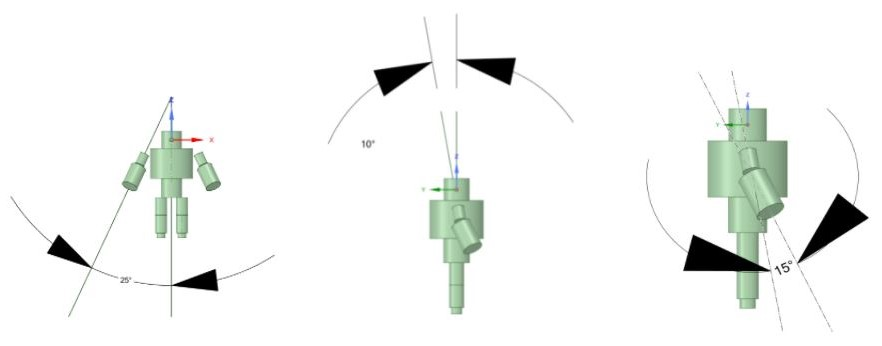
\includegraphics[width=\columnwidth]{./imagines/model_cad.JPG}
%     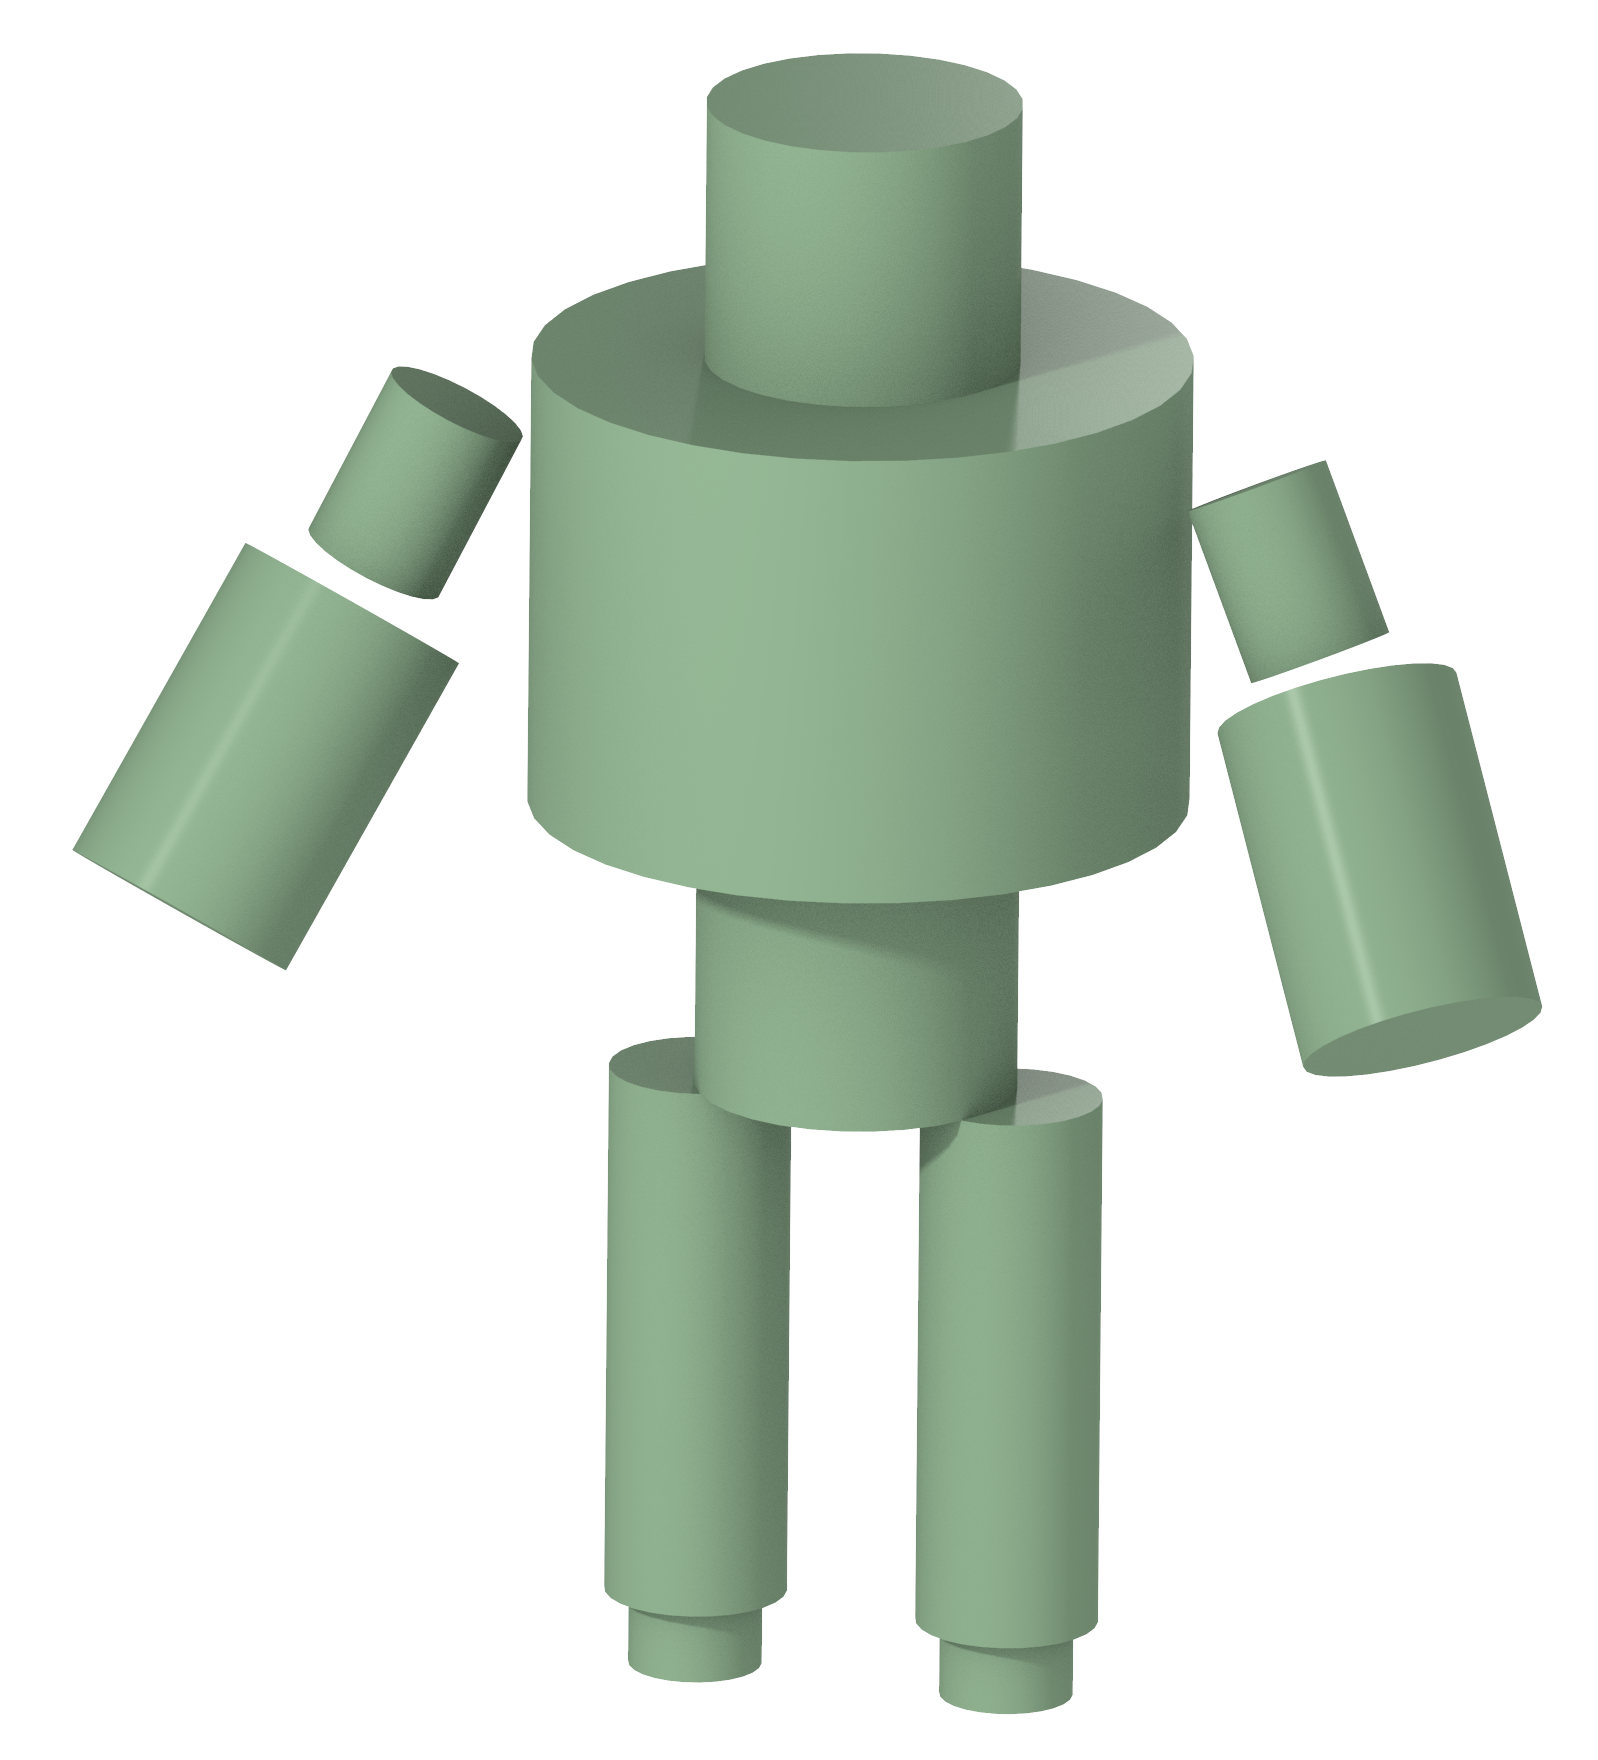
\includegraphics[width=\columnwidth]{./imagines/ironcub-cfd-3d.png}
      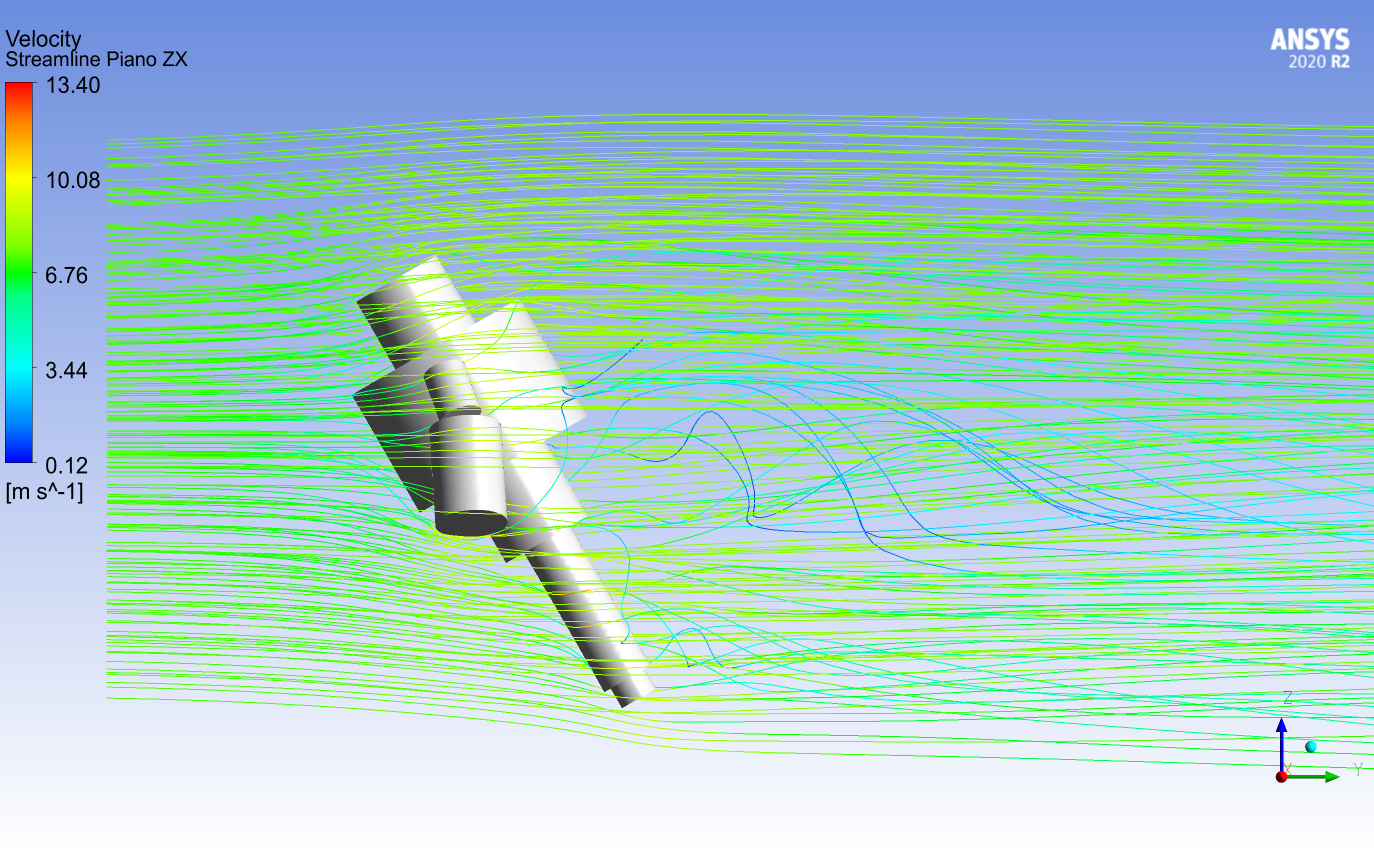
\includegraphics[width=50mm]{./imagines/cfd_simu.png}
      \caption{CFD simulation using simplified iRonCub CAD model: initial joint configuration.}
      \label{fig:cad}
   \end{figure}
\end{comment}
 % The robot shape under the chosen initial joint configuration  is referred to generate the simplified CAD model used in CFD simulations, see Fig. \ref{fig:cad}. Robot's joint configuration may vary while proceeding different flying tasks which leads to the change of robot shape. However, by means the \textit{postural task} in our previous work \cite{c1}\cite{c2}, the robot joint configuration is kept close to the initial one. Different robot shape in CFD simulations provides different results which influences also the analytical models built based on the CFD data, however, the variation is neglected due to the fact that the joint movements are small enough, i.e. the robot shape almost remains unchanged in the studied flight envelope.
 
\subsection{Aerodynamic components for CFD analysis}
\label{sec:cfd} 
 
%We prefer to model the \emph{global} aerodynamic force acting on the robot, because evaluating aerodynamic effects distributed on several parts of the body requires to design a more complex robot model for the CFD analysis, which becomes very time consuming. \fabioDsays{Probably here we can justify the use of the simplified model saying that the main goal is to validate the procedure} The global aerodynamic effects at the robot CoM are composed of the aerodynamic force ${F}_a \in \mathbb{R}^3$, and the moment ${M}_a:={\mathcal{G}P}\times {F}_a \in \mathbb{R}^3$, where ${\mathcal{G}P}$ is the distance between the CoM $\mathcal{G}$ and the Center of Pressure (CoP) $P$. 

%\antonellosays{From here on probably we should rewrite the modeling to take into account for the [14] notation.}

For the sole purpose of CFD analysis, let us introduce the frame $\mathcal{A}=\{{}^{\mathcal{I}}o_{\mathcal{G}};\boldsymbol{i}_a,\boldsymbol{j}_a,\boldsymbol{k}_a\}$ as the \emph{relative velocity} frame. It is defined for CFD simulations only, where the relative velocity is always different from zero, namely $|\boldsymbol{v}_a|\neq 0$. 
%The relative velocity frame  to map the aerodynamic forces values as functions of $\alpha$ and $\beta$ angles. 
%The axes are defined starting from $\mathcal{D}$, with a \textit{ZXZ} frame rotation of $\left\{\beta - \frac{\pi}{2};\ \alpha + \frac{\pi}{2};\ 0\right\}$ with $\alpha$ and $\beta$ defined as in \ref{sec:af}. 
The $\boldsymbol{j}_a$ axis therefore aligns to the opposite direction of $\boldsymbol{v}_a$ (see also Fig. \ref{figureRelativeVelocityFrameCFD}).

\begin{figure}[t]
      \centering
      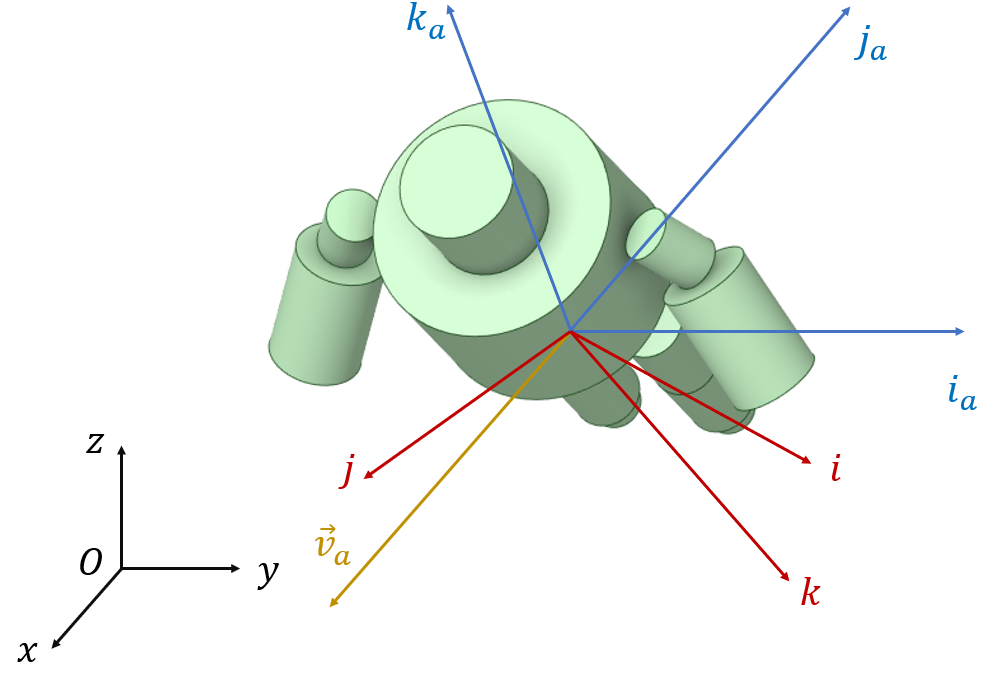
\includegraphics[width=60mm]{./imagines/CFD_Reference_System_3.png}
      \caption{CFD Model with the relative velocity frame.}
      \label{figureRelativeVelocityFrameCFD}
   \end{figure}

Then, we decompose the aerodynamic force w.r.t. the relative velocity frame $\mathcal{A}$ as:
\begin{equation}
\label{eq:af_total_control}
\boldsymbol{{F}_a}=\boldsymbol{{F}_D}+\boldsymbol{{F}_S}+\boldsymbol{{F}_N} ,
\end{equation}
where:
\begin{itemize}
    \item $\boldsymbol{{F}_D}$, the drag force, aligns to $\boldsymbol{j}_a$ axis;
    \item $\boldsymbol{{F}_S}$, the defined sideforce, aligns to $\boldsymbol{i}_a$ axis;
    \item $\boldsymbol{{F}_N}$, the defined normal force, aligns to $\boldsymbol{k}_a$ axis.
\end{itemize}
The intensity of the steady aerodynamic force varies approximately with $|\boldsymbol{v}_a|^2$, hence there exist three dimensionless functions $C_D$, $C_S$, $C_N$ depending on the Reynolds number $Re$, the Mach number $\mathcal{M}$ and $(\alpha, \beta)$, such that \cite{c3}\cite{c5}:
\begin{subequations}
\begin{align}
    \boldsymbol{{F}_D} & :=\mathcal{K}_a|\boldsymbol{v}_a|^2C_D(Re, \mathcal{M}, \alpha, \beta)\boldsymbol{j}_a,\\
    \boldsymbol{{F}_S} & :=\mathcal{K}_a|\boldsymbol{v}_a|^2C_S(Re, \mathcal{M}, \alpha, \beta)\boldsymbol{i}_a,\\
    \boldsymbol{{F}_N} & :=\mathcal{K}_a|\boldsymbol{v}_a|^2C_N(Re, \mathcal{M}, \alpha, \beta)\boldsymbol{k}_a,
\end{align}
\label{eq:af_coe}
\end{subequations}
\noindent with the angles $(\alpha, \beta)$ characterizing the relative orientation of $\boldsymbol{v}_a$ w.r.t. the body frame $\mathcal{D}$, chosen as in  Fig.~\ref{fig:notation}. So, $\alpha \in [0,\pi]$ is defined as the angle between $\boldsymbol{v}_a$ and the negative $\boldsymbol{k}$ axis of the body frame $\mathcal{D}$, while $\beta \in [0,2\pi]$ is defined as the angle between the projection of $\boldsymbol{v}_a$ on plane $(\boldsymbol{i},\boldsymbol{j})$ and the positive $\boldsymbol{i}$ axis of frame $\mathcal{D}$ (see also \cite{c3}). The constant $\mathcal{K}_a:=\frac{A_{ref}\rho}{2}$ with $\rho$ the air density and $A_{ref}$ the reference frontal area, moreover, $A_{ref}$ has been defined to obtain $\mathcal{K}_a = 1$ to simplify the calculation. Furthermore, we hereafter assume that the dependency upon the Mach and Reynolds numbers is negligible, and thus omitting these dependencies in the arguments of the aerodynamic coefficients. 
%$\boldsymbol{i}_a$, $\boldsymbol{j}_a$, $\boldsymbol{k}_a$ are the unit vectors of frame $\mathcal{A}$ along $\boldsymbol{X}_a$, $\boldsymbol{Y}_a$, $\boldsymbol{Z}_a$ axes.
%In particular, $\boldsymbol{j}_a$ has the opposite direction of $\boldsymbol{v}_a$ by definition. Identifying the numerical relation among the dimensionless coefficients $C_D$, $C_S$, $C_N$ and their variables is fundamental for the design of analytical models of the aerodynamic forces to be in the system modeling and control design. 

%\fabioDsays{The AC model should be changed according to the new axes references, as also Antonello said.}

\subsection{CFD results and simplified aerodynamic model}\label{sec:aeroModel}

Significant robot flight configurations, corresponding to precise values of $\alpha$ and $\beta$, were simulated using CFD tools. In total 45 simulations were run, with $ \alpha \in (\ang{15},\ \ang{30},\ \ang{45},\ \ang{60},\ \ang{90},\ \ang{120},\ \ang{150},\ \ang{160},\ \ang{180})$ and $ \beta \in (\ang{90},\ \ang{135},\ \ang{180},\ \ang{225},\ \ang{270})$ which supplied the necessary data for proceeding with the modeling of aerodynamic characteristics on iRonCub. Settings of CFD simulations are schematically reported in Table \ref{table:cfd}.
% In particular, by assuming the flow density as constant (valid hypothesis due to the not extremely high flight speed and the absence of heat sources) the computational cost is reduced since the Energy equation has not to be solved.
 
% Another angle pair $(\alpha_{cfd},\beta_{cfd})$ is defined for CFD simulations only to set the relative orientation between the flow and the robot, where $\alpha_{cfd}=90^{\circ} -\alpha$, $\beta_{cfd}=180^{\circ}-\beta$. By importing different values of $\alpha_{cfd}$ and $\beta_{cfd}$ (see Table \ref{table:Sim_cases}), in total $21$ simulations are completed which supply data for aerodynamic modeling on iRonCub.
 
\begin{comment}
\begin{table}[t]
\caption{CFD simulation settings}
\label{table:cfd}
\begin{center}
\begin{tabular}{|c|m{15em}|}
\hline
\multirow{4}{*}{\textit{Solver Settings}} & Pressure--Velocity Coupling for \emph{RANS} (Reynolds Averaged Navier-Stokes) \\ & Steady-State Simulation\\ & SST k - $\omega$ for Turbulence modelling \\ & No Compressibility Effects (i.e. $M<<1$, $\rho = const$)\\
\hline
\multirow{2}{*}{\textit{Constant Values}} & Air density: $\rho = 1.225 \ kg/m^3$ \\ & Reference pressure: $p_{ref} = 1 \ atm$\\
\hline
\multirow{3}{*}{\textit{Boundary Conditions}} & Inlet velocity: $v = 7.5 \ m/s$ \\ & Outlet pressure: $p_{rel} = 0 \ Pa$\\ & Walls: \textbf{No Slip} Condition\\
\hline
\end{tabular}
\end{center}
\end{table}
\end{comment}

\begin{table}[t]
\caption{CFD simulation settings}
\label{table:cfd}
	\centering
	\begin{tabular}{c|l}
	    \toprule
	    \multirow{6}{*}{\textit{Solver Settings}} & Pressure--Velocity Coupling for \emph{RANS} \\ & (Reynolds Averaged Navier-Stokes) \\ & Steady-State Simulation\\ & SST $k - \omega$ for Turbulence modelling \\ & No Compressibility Effects \\ & (i.e. $M\ll1$, $\rho = \text{const}$)\\
		\midrule
		\multirow{2}{*}{\textit{Constant Values}} & Air density: $\rho = \SI{1.225}{kg/m^3}$ \\ & Reference pressure: $p_{ref} = \SI{1}{atm}$\\
        \midrule
        \multirow{3}{*}{\textit{Boundary Conditions}} & Inlet velocity: $v = \SI{7.5}{m/s}$ \\ & Outlet pressure: $p_{rel} = \SI{0}{Pa}$\\ & Walls: \textbf{No Slip} Condition\\
		\bottomrule
	\end{tabular}
\end{table}

%Another angle pair $(\alpha_{cfd},\beta_{cfd})$ is defined for CFD simulations, which specifies the relative orientation between the flow and the robot. It holds that $\alpha_{cfd}=90^{\circ} -\alpha$ and $\beta_{cfd}=180^{\circ}-\beta$. 
 \looseness=-1

\begin{comment}
\begin{table}[t]
\caption{Simulations Table}
\label{table:Sim_cases}
\begin{center}
\begin{tabular}{|c|c|c|c|c|c|c|}
\hline
\multicolumn{2}{|c|}{} & \multicolumn{5}{c|}{$ \beta $} \\
\cline{3-7}
\multicolumn{2}{|c|}{} & \multicolumn{1}{c|}{180} & \multicolumn{1}{c|}{225} & \multicolumn{1}{c|}{270} & \multicolumn{1}{c|}{315} & \multicolumn{1}{c|}{360}\\
\hline
\multicolumn{1}{|c|}{} & \multicolumn{1}{c|}{15} & \multicolumn{1}{c|}{} & \multicolumn{1}{c|}{} &  \multicolumn{1}{c|}{\checkmark} & \multicolumn{1}{c|}{} & \multicolumn{1}{c|}{}\\
\cline{2-7}
\multicolumn{1}{|c|}{} & \multicolumn{1}{c|}{30} & \multicolumn{1}{c|}{\checkmark} & \multicolumn{1}{c|}{} & \multicolumn{1}{c|}{} & \multicolumn{1}{c|}{} & \multicolumn{1}{c|}{}\\
\cline{2-7}
\multicolumn{1}{|c|}{} & \multicolumn{1}{c|}{45} & \multicolumn{1}{c|}{} & \multicolumn{1}{c|}{} & \multicolumn{1}{c|}{\checkmark} & \multicolumn{1}{c|}{} & \multicolumn{1}{c|}{}\\
\cline{2-7}
\multicolumn{1}{|c|}{} & \multicolumn{1}{c|}{60} & \multicolumn{1}{c|}{\checkmark} & \multicolumn{1}{c|}{\checkmark} & \multicolumn{1}{c|}{\checkmark} & \multicolumn{1}{c|}{\checkmark} & \multicolumn{1}{c|}{\checkmark}\\
\cline{2-7}
\multicolumn{1}{|c|}{$ \alpha $} & \multicolumn{1}{c|}{90} & \multicolumn{1}{c|}{\checkmark} & \multicolumn{1}{c|}{\checkmark} & \multicolumn{1}{c|}{\checkmark} & \multicolumn{1}{c|}{\checkmark} & \multicolumn{1}{c|}{\checkmark}\\
\cline{2-7}
\multicolumn{1}{|c|}{} & \multicolumn{1}{c|}{120} & \multicolumn{1}{c|}{\checkmark} & \multicolumn{1}{c|}{\checkmark} & \multicolumn{1}{c|}{\checkmark} & \multicolumn{1}{c|}{\checkmark} & \multicolumn{1}{c|}{\checkmark}\\
\cline{2-7}
\multicolumn{1}{|c|}{} & \multicolumn{1}{c|}{150} & \multicolumn{1}{c|}{\checkmark} & \multicolumn{1}{c|}{} & \multicolumn{1}{c|}{} & \multicolumn{1}{c|}{} & \multicolumn{1}{c|}{}\\
\cline{2-7}
\multicolumn{1}{|c|}{} & \multicolumn{1}{c|}{160} & \multicolumn{1}{c|}{} & \multicolumn{1}{c|}{} & \multicolumn{1}{c|}{\checkmark} & \multicolumn{1}{c|}{} & \multicolumn{1}{c|}{}\\
\cline{2-7}
\multicolumn{1}{|c|}{} & \multicolumn{1}{c|}{180} & \multicolumn{1}{c|}{} & \multicolumn{1}{c|}{} & \multicolumn{1}{c|}{\checkmark} & \multicolumn{1}{c|}{} & \multicolumn{1}{c|}{}\\
\hline
\end{tabular}
\end{center}
\end{table}
\end{comment}


%\begin{table}[t]
%\vspace*{0.3cm}
%\caption{Simulations Table}
%\label{table:Sim_cases}
%\begin{center}
%\rowcolors{2}{white}{gray!15}
%\begin{tabular}{c|c|c|c|c|c}
%\toprule
%\diagbox[width=6em]{$\alpha[\degree]$}{$\beta[\degree]$} & {180} & {225} & {270} & {315} & {360}  \\
%\midrule
%{15} & {} & {} &  {\checkmark} & {} & {}\\
%{30} & {\checkmark} & {} & {} & {} & {}\\
%{45} & {} & {} & {\checkmark} & {} & {}\\
%{60} & {\checkmark} & {\checkmark} & {\checkmark} & {\checkmark} & {\checkmark}\\
%{90} & {\checkmark} & {\checkmark} & {\checkmark} & {\checkmark} & {\checkmark} \\
%{120} & {\checkmark} & {\checkmark} & {\checkmark} & {\checkmark} & {\checkmark}\\
%{150} & {\checkmark} & {} & {} & {} & {}\\
%{160} & {} & {} & {\checkmark} & {} & {}\\
%{180} & {} & {} & {\checkmark} & {} & {}\\
%\bottomrule
%\end{tabular}
%\end{center}
%\end{table}



As introduced in Sec. \ref{sec:cfd}, the three dimensionless functions $C_D$, $C_S$, $C_N$ are the aerodynamic characteristics of the body, i.e. the defined aerodynamic coefficients (AC): drag coefficient, sideforce coefficient and normal force coefficient. In this section, the analytical model of AC is identified based on the CFD results from Sec. \ref{sec:cfd}. To proceed with identification, the following assumptions are made:

\begin{enumerate}
\item the aerodynamic forces act at the robot's CoM (coincides with CoP) and therefore the aerodynamic moments ${M}_a$ are equal to zero;
\item from CFD results, the sideforce effect is neglected due to its small magnitude compared with the other two aerodynamic force components, and with other forces acting on the robot;
\item the AC dependence from Mach number $\mathcal{M}$ is considered negligible since the relative velocity intensity of the robot is much smaller than the sound speed (i.e. the density can be assumed as constant);
\item the AC dependence from Reynolds number $Re$ is not considered since the AC evaluated from CFD for different values of relative velocity doesn't show a significant dependence from it;
\item the effects of rotational and unsteady motions of the vehicle on its surrounding airflow are negligible~\cite{c5}.
\end{enumerate}

As a consequence, the AC depend only on the flight configuration $(\alpha,\beta)$ and can be written as~\cite{c3}:
\begin{equation*}
    C_D(\cdot) =C_D(\alpha, \beta), \quad  C_N(\cdot) =C_N(\alpha, \beta) .
\end{equation*}
%C_S(\cdot)& =C_S(\alpha, \beta) , 
%Exporting aerodynamic forces from the aforementioned CFD analysis, the estimated sideforce is up to $1.68 \ N$ with the air speed (wind speed) of $7.5 \ m/s$ which is relatively small compared with the other two aerodynamic force components (over $10 \ N$ ) and the magnitude of other forces acting on the robot (gravity force of iRonCub is around $400 \ N$, thrust force of each engine is around $200 \ N$). Thus, we neglect the sideforce and the paper work contributes to the model identification of drag force coefficient $C_D(\cdot)$ and normal force coefficient $C_N(\cdot)$.
%(more than $\SI{10}{N}$ each) 
%(e.g. the gravity force of the whole robot is around $\SI{400}{N}$)
% The estimated sideforce from CFD results (with air speed as $\SI{7.5}{m/s}$) reaches a maximum value of $\SI{1.68}{N}$, which is relatively small compared with the other two aerodynamic force components or with other forces acting on the robot. It is thus possible to neglect the effect due to sideforce, and focus on the model identification of $C_D(\cdot)$ and $C_N(\cdot)$.
Considering that the aerodynamic coefficients are naturally $2\pi$-periodic \cite{c12}, $\sin{(\cdot)}$ functions are used to design the mathematical models of AC: %, which are hereafter displayed:
\begin{equation}
    \resizebox{.88 \columnwidth}{!}{$ 
        C_D(\alpha,\beta)= c_0 + c_1 \sin{^2 \alpha} \sin{^2\beta} + c_2 \sin{^2\alpha}  + c_3 \sin{^2\beta}
    $},\label{eq:drag}
 \end{equation}
 \begin{equation}
    C_N(\alpha,\beta)= d_0 + d_1 \sin{^2\alpha} \sin{(2\alpha)} \sin{^2\beta} .
    \label{eq:normal}
 \end{equation}

% \begin{multline}
%     C_D(\alpha,\beta)=c_0+c_1sin^2(\alpha)cos^3(\beta)+c_2cos^3(\beta)  \\
%     +c_3cos^2(\beta) ,
%  \end{multline}
%  \begin{equation}
%     C_N(\alpha,\beta)=d_0+d_1sin(2\alpha)cos^2(\beta) .
%  \end{equation}

The coefficients characterizing the expressions of $C_D(\cdot)$ and $C_N(\cdot)$:
\begin{itemize}
    \item $c_0=0.1274$, $c_1=0.0903$, $c_2=0.0141$, $c_3=0.0147$;
    \item $d_0=0.0007$, $d_1=0.0938$,
\end{itemize}
\noindent
are obtained using linear regression. \\
In fluid dynamics, drag force is a type of friction that acts in the opposite direction of the relative motion of any object moving in a fluid. Therefore the estimated drag coefficient $C_D$ should remain positive in the whole range of $\alpha$ and $\beta$. This property is verified by the identified model in Eq.~\eqref{eq:drag}, as Fig.~\ref{fig:drag model} shows.

As previously mentioned, the zero sideforce assumption allows the identification of the lift force with the normal force, as demonstrated in~\cite{c3} for axisymmetric bodies, since the normal component of the aerodynamic force lies on the $\boldsymbol{v}_a-\boldsymbol{k}_a$ plane. The aerodynamic forces acting on the robot CoM rewrite as:

\begin{equation}
\label{eq:aerodyModelSymmetricBodies}
\begin{array}{lcl}
	\boldsymbol{F_L} & = & k_a|\boldsymbol{v}_a|C_L(\alpha,\beta)\boldsymbol{r}(\beta) \times \boldsymbol{v}_a, \\
	\boldsymbol{F_D} & = & -k_a |\boldsymbol{v}_a|C_D(\alpha,\beta)\boldsymbol{v}_a, \\
\end{array}
\end{equation}
where  $\label{eq:aerodynamicsAuxiliaryVector}
\boldsymbol{r}(\beta)  =  -\sin(\beta) \boldsymbol{i}+\cos(\beta) \boldsymbol{j}.$

 \begin{figure}[t]
\centering
\subfigure[\label{fig:drag model}]{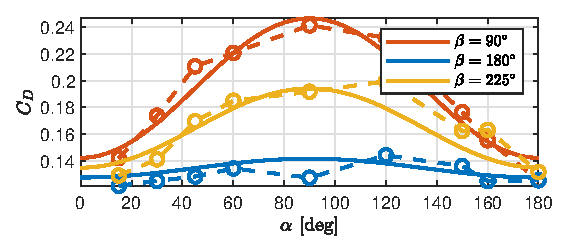
\includegraphics[width=0.97\columnwidth]{imagines/pics_v2/Cd_alpha.eps}}\\
\subfigure[\label{fig:normal model}]{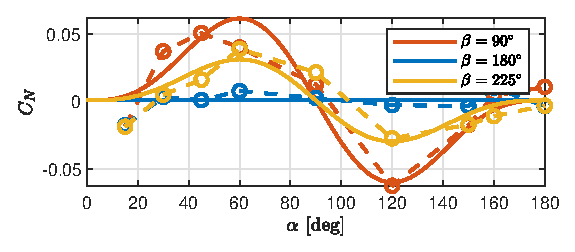
\includegraphics[width=0.97\columnwidth]{imagines/pics_v2/Cn_alpha.eps}} \\
\caption{AC models identified from CFD simulations data. Dashed lines represent the collected CFD data, solid lines represent the identified models.}
\label{fig:subfig}
\end{figure}

\section{Control Design}
\label{sec:control}

%\fabioDsays{Could we add here some brief notions on control methods?}

\subsection{Flight Control Without Aerodynamics Awareness}
\label{subsec:Flight-Control-no-aerodyn-forces}
The iRonCub flight controller~\cite{c1, c2} is a \emph{task-based} control strategy, composed of several control objectives (tasks), with different priorities. The so-called \emph{primary task}, i.e. the task with the higher priority, is the stabilization of the robot's \emph{centroidal momentum}\footnote{The centroidal momentum is the robot total momentum expressed w.r.t. the frame $\mathcal{G}[\mathcal{I}]$  defined in Sec. \ref{background}.} dynamics, which equals the summation of all external forces acting on the robot:
%
\begin{equation}
\label{eq:hdot}
   {}^{\mathcal{G}[\mathcal{I}]}\dot{\boldsymbol{h}}=\boldsymbol{A}(q)T+m\bar{\boldsymbol{g}}=f_h(q,T),
\end{equation}

%change f(q,T) to f_h(q,T), because f has been used as trust function, $g$ is the norm of gravitational acceleration and 
where $m$ is the robot's total mass, $\boldsymbol{A}(q) \in \mathbb{R}^{6 \times m}$ is a proper matrix mapping the thrust vector $T$ in the momentum equation. For the momentum control design, we assume that the robot joints velocities $\dot{s}$ and the thrust rate of change $\dot{T}$ can be chosen at will, and then can be considered as our control inputs. Therefore, we define $u := (\dot{T}, \dot{s})$. To make the control input $u$ appear in the momentum equation \eqref{eq:hdot}, we increase the relative degree of the output and write the momentum acceleration:
%
\begin{equation}
\label{eq:hddot}
   {}^{\mathcal{G}[\mathcal{I}]}\ddot{\boldsymbol{h}}=\dot{\boldsymbol{A}}(q)T+\boldsymbol{A}(q)\dot{T} = f_h(q, T, v, \dot{T}).
\end{equation}
%
As demonstrated in our previous works \cite{c1,c2}, it is possible to find a smooth control input $u^*$ that renders the closed-loop equilibrium point $(\dot{\tilde{\boldsymbol{h}}}, \tilde{\boldsymbol{h}}, \boldsymbol{I}) = (\boldsymbol{0},\boldsymbol{0},\boldsymbol{0})$ globally asymptotically stable, where $\tilde{\boldsymbol{h}} = \boldsymbol{h}-\boldsymbol{h}^d$, $\boldsymbol{h}^d$ is the reference momentum trajectory and $\boldsymbol{I} := \int_0^t \tilde{\boldsymbol{h}}$. 

We also define a \emph{postural task} to resolve the redundancy in the control input $u$ and maintain the robot configuration close to a desired shape:
%
\begin{equation}
\label{eq:postural}
   \dot{s}^* = -K_P^s (s-s^d),
\end{equation}
%
with $s^d$ the desired robot posture and $K_P^s \in \mathbb{R}^{n \times n}$ a positive gains matrix. The two tasks are then achieved by means of Quadratic Programming (QP) optimization framework:
\begin{IEEEeqnarray}{LLL}
\IEEEyesnumber
\label{eq:optimization_QP}
   u^{**} &=& \text{argmin}_{u} (w_1|u-u^*|^2 + w_2|\dot{s}-\dot{s}^*|^2) \\
     & s.t. & \qquad u_{min} \leq u \leq u_{max}, \nonumber
\end{IEEEeqnarray}
where \emph{soft} task priorities are assigned to the two tasks via proper weights $w_1, w_2 >0$. Framing the problem as an optimization procedure allows to include input boundaries $u_{min}, u_{max}$ in the control design. It is also possible to include the integral of input boundaries (namely, the joint position and thrust limits) in the QP design. For more details on these aspects of the flight control design, which are not relevant for this paper, we refer to previous works \cite{c1,c2}.

\subsection{Flight Control with Aerodynamics Awareness}

The flight controller discussed in \ref{subsec:Flight-Control-no-aerodyn-forces} does not consider the effect of aerodynamic forces. This missing information may impair the performances of the control algorithm when aerodynamic forces are not negligible. To overcome this limitation, we implemented two modifications of the iRonCub flight controller: \emph{feedback linearization} and \emph{gain scheduling}.
To implement our control strategy, we considered the following \textbf{Assumption 2}: we assume that $\dot{\boldsymbol{F}}_a = 0$ in the calculation of the momentum acceleration.

% \begin{itemize}
% \item we assume that $\dot{F}_a = 0$ in the calculation of the momentum acceleration.
% \end{itemize}
\subsubsection*{Addition of Aerodynamics Forces}
First, we include the estimated aerodynamic forces, obtained by writing Eq. \eqref{eq:af_total_control} with the aerodynamic coefficients estimated in Sec. \ref{sec:aeroModel}, in the robot equations of motion Eq. \eqref{eq_motion} and momentum dynamics Eq. \eqref{eq:hdot}, which renders:
\begin{equation}
\label{eq_motion_af}
  M(q)\dot{v}+C(q,v)v+G(q)=
  \begin{bmatrix}
    0_6\\
    \tau
  \end{bmatrix}
  +f(q,T)+J_{CoM}^{\top}F_a,
\end{equation}
where $J_{CoM} \in \mathbb{R}^{3 \times n+6}$ is the CoM Jacobian, while the momentum rate of change is now given by:
\begin{equation}
\label{eq:hdot_af}
   {}^{\mathcal{G}[\mathcal{I}]}\dot{\boldsymbol{h}}=\boldsymbol{A}(q)T+m\bar{\boldsymbol{g}}+
   \begin{bmatrix}
   \boldsymbol{F_a}\\
   0_3
   \end{bmatrix}.
\end{equation}

\subsubsection*{Feedback Linearization Control}

We assume that the relative velocity ${}^{\mathcal{I}}\boldsymbol{v}_a$ can be measured, for example by employing dedicated sensors such as Pitot tubes applied on the robot, allowing the computation of the aerodynamic force $F_a$. A feedback linearization controller then substitutes Eq.~\eqref{eq:hdot} with Eq.~\eqref{eq:hdot_af} in the calculation of the baseline control input $u^*$, which depends on the momentum rate of change $\dot{h}$. In this way we can cancel out the effects of the aerodynamic forces on the desired closed-loop momentum acceleration.

\subsubsection*{Implementation of Gain Scheduling}
%Two flying conditions - hovering and high-speed flight - of the robot are studied. The linear velocity of the robot's CoM point ${}^{\mathcal{I}}\boldsymbol{v}_{CoM}$ reaches around $\SI{11}{m/s}$ during the high-speed flight along the $+\boldsymbol{X}$ axis of the inertial frame $\mathcal{I}$, see Appendix \ref{appendix:traj}. The simulated air environment for control design is represented by a constant wind speed of $\SI{3}{m/s}$, strengthened by a wind gust lasting $5$ seconds, see Fig. \ref{fig:wind}. The wind velocity ${}^{\mathcal{I}}\boldsymbol{v}_w$ has the direction along the $-\boldsymbol{X}$ axis of the inertial frame $\mathcal{I}$ and this direction is tested via simulations to be more critical for both hovering and high-speed flight cases, i.e. the aerodynamic effects on the system are stronger. 

if it is not possible to compute the aerodynamic forces with enough accuracy, gain scheduling is employed as a strategy to react to wind gusts. In particular, we assume that a wind gust is detected when the measured center of mass position error overcomes a certain threshold.

The desired closed-loop momentum acceleration has the following shape, which is obtained by applying the baseline controller $u^*$ Eq. \eqref{eq:optimization_QP}:
\begin{equation}
\label{eq:hddot_des}
   \ddot{\boldsymbol{h}} = \ddot{\boldsymbol{h}}^d -K_D\dot{\tilde{\boldsymbol{h}}} -K_P\tilde{{\boldsymbol{h}}} -K_I \boldsymbol{I}.
\end{equation}
When a wind gust is detected, gain scheduling smoothly increases the value of the gain $K_I$ and $K_P$, to guarantee a stronger response of the controller to the associated errors.

%A simple method to deal with multiple operating conditions caused by aerodynamic effects under the wind gust impact is to apply the gain-scheduling technique. Ensuring the aforementioned main control objectives, the gain-scheduling applies on the proportional gains $K_p=[K_{px} \ K_{py} \ K_{pz}]$ that are related to the CoM position. \giusesays{Maybe write here or in the controller section the formula that describes the desired closed loop com dynamics}.\tongsays{need to confirm with Gabri how to arrange the parts for current controller}

%In hovering condition, the aerodynamic effects cause big CoM position error during the wind gust impact (see Fig. \ref{fig:h_rob}) but the robot can stabilize even with fairly high wind gust value (up to $\SI{53}{m/s}$), and thus we aims at reducing the CoM position error by increasing the gain values (starting from $15$) when wind gust appears, see Fig. \ref{fig:raise gain}. In high-speed flight condition, however, due to the high magnitude of the relative velocity, the strong aerodynamic effects lead to instability  (see Fig. \ref{fig:hf_rob}) of the robot when the wind gust value is over $\SI{9}{m/s}$. To stabilize the robot, we reduce the gain values (starting from $15$) during wind gust impact period, see Fig. \ref{fig:raise gain}.
%\fabioDsays{Can't we reduce this paragraph just saying that the way we applied gain scheduling may differ according to the simulated scenario and move the references to the results in the Simulation Validation Section?} \fabioBsays{I agree}

%\begin{figure}[b]
%    \centering
%        \subfigure[]{\label{fig:a}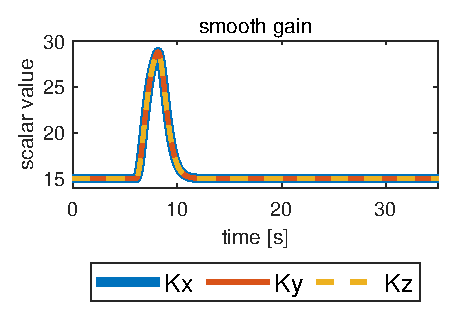
\includegraphics[width=40mm]{./imagines/smooth_gain_2h.eps}}
%        \subfigure[]{\label{fig:b}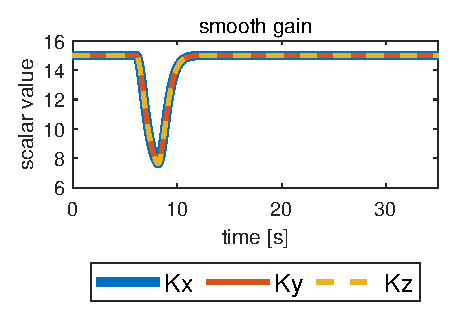
\includegraphics[width=40mm]{./imagines/smooth_gain_1f.eps}}
%    \caption{Gain-scheduling: a) for hovering; b) for high-speed flight. $K_x, K_y, K_z \in \mathbb{R}^+$ are the elements along the diagonal of matrix $K_I$.} 
%    \label{fig:raise gain}
%\end{figure}

%Besides the implementation of feedback law on momentum dynamics, the aerodynamic forces are also considered in the torque controller \cite{c1}\cite{c2} for joint dynamics according to the change of the system equations of motion in Eq. \ref{eq_motion_af}, see Appendix \ref{appendix:joint}. \fabioDsays{not super clear this last sentence. My understanding is that "for joint dynamics" we modified the equations "in a similar way to what done in Eq. 6."}